\chapter{Configuring JEGA} \label{ch:configuration}

There are two conceptually different types of configuration to be
discussed in this chapter.  The first involves how to configure the
source code when compiling JEGA.  The second is how to configure
JEGA to perform operations the way you want at run time.

\section{Compile Time Configuration Options}\label{sec:compile_config}

JEGA is distributed as source code and thus, it must be compiled
prior to being used.  The following sections describe the various
compile time options that are available with JEGA and how to use
them.

\subsection{Compiler Specification}\label{sec:compiler_specification}

You can specify to the configure utility which C++ compiler to use
by providing a value for the CXX variable on the command line.  You
can specify flags to be passed to the compiler by providing a value
for the CXXFLAGS variable on the command line.  For example, suppose
your default compiler is g++ 3.4 and you wish to use 4.0 and build
with debugging information.  The configuration command line would
look like:

\texttt{>> \$(JEGA\_ROOT)/configure CXX=/usr/local/bin/g++4 CXXFLAGS=-g}

\subsection{Logging}\label{sec:compile_logging_config}

As discussed in Section~\ref{sec:logging}, JEGA is capable of
logging status messages describing the workings of the various
algorithmic components, the progression of the algorithm, etc.  This
behavior can be controlled in part during compilation of JEGA.  JEGA
supports logging to the console window using the standard output
stream (cout for C++ programmers) and to a file with a name that can
be specified programmatically at configuration time.

By default, JEGA will do no logging whatsoever.  To enable logging,
the preprocessor constant \texttt{JEGA\_LOGGING\_ON} must be defined
for your project.  This is typically accomplished by modifying make
files and/or project files.  If you are using the autoconf harness
distributed with JEGA then logging is on by default and can be
disabled by passing the optional flag \texttt{--disable-logging} at
configuration time.

If you wish to log to only one or the other of the console and file
you can optionally define constants to disable the other.  They are
\texttt{JEGA\_LOGGING\_NO\_CONSOLE} and
\texttt{JEGA\_LOGGING\_NO\_FILE} respectively. These constants must
be defined along with \texttt{JEGA\_LOGGING\_ON}. Defining either of
these without defining \texttt{JEGA\_LOGGING\_ON} will have no
effect and no logging will occur. Defining both of these will result
in no logging regardless of whether or not you've defined
\texttt{JEGA\_LOGGING\_ON}.  If using the autoconf harness, then the
options \texttt{--enable-logging-no-console} and
\texttt{--enable-logging-no-file} can be used to achieve the desired
effect.

To summarize, if you wish to do no logging, do not define
\texttt{JEGA\_LOGGING\_ON}.  If you wish to log to both the console
window and to a file, define \texttt{JEGA\_LOGGING\_ON}.  If you
wish to log to only the console window, define
\texttt{JEGA\_LOGGING\_ON} and \texttt{JEGA\_LOGGING\_NO\_FILE}.
Finally, if you wish to log only to a file and not to the console
window, define \texttt{JEGA\_LOGGING\_ON} and
\texttt{JEGA\_LOGGING\_NO\_CONSOLE}.

\subsection{Debugging}\label{sec:compile_debugging_config}

If distributed under the LGPL, GPL, or certain other open source
licenses, JEGA comes equipped with a very simple but powerful
debugging capability.  A great deal of source code exists in the
JEGA project to support the use of this facility.  This code checks
for exceptional, unusual, or erroneous conditions.  If such a
condition is found, the debugging code causes an assertion failure
along with a rudimentary scope trace.  The same scope trace will
appear if a signal is caught with a description of the signal if it
is known.  Figure~\ref{fig:JEGA_debug_scope_trace} below shows what
one might see if a segmentation fault occurs during JEGA execution.

\begin{figure}[!ht]
    \centering
    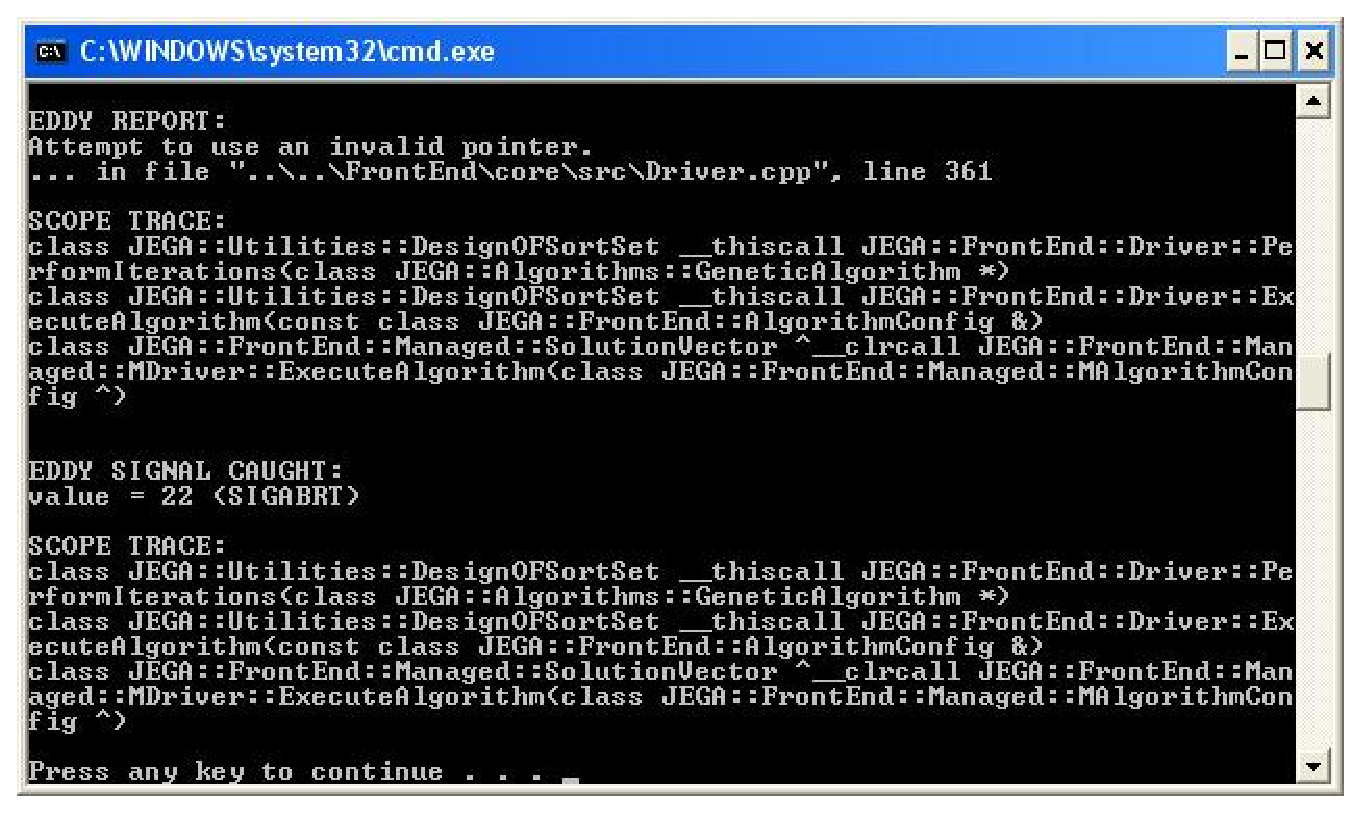
\includegraphics[scale=0.70]{../../images/scope_trace.eps}
    \caption{Example JEGA Debug Scope Trace}
    \label{fig:JEGA_debug_scope_trace}
\end{figure}

This capability is disabled by default.  To enable it, you must
define the \texttt{JEGA\_OPTION\_DEBUG} preprocessor constant on
your compiler command line or in your project files.  If using the
autoconf harness that is distributed with JEGA, then you may supply
the optional \texttt{--enable-debugging} flag during the
configuration step to enable debugging.

Compiling with this option will add a fair amount of additional code to your assembly and slow down your execution.  It is therefore only recommended as a debugging tool if you are having problems.

\subsection{Thread Safety}\label{sec:compile_threading}

As discussed in Section~\ref{sec:thread_safety}, JEGA can be
configured to run in a thread safe manner.  This allows multiple
JEGA algorithms to be run in order to solve the same problem
simultaneously from separate threads. This behavior can be
controlled only during compilation of JEGA.

By default, JEGA will will not compile with thread safe behavior. To
enable thread safety, the preprocessor constant
\texttt{JEGA\_THREADSAFE} must be defined for your project.  This is
typically accomplished by modifying make files and/or project files.
If you are using the autoconf harness distributed with JEGA then
thread safety can be enabled by passing the optional flag
\texttt{--enable-threadsafe} at configuration time.

Note that this feature is not only relevant to the running of multiple concurrent algorithms, but also to the ability for JEGA evaluators to perform concurrent evaluations using multiple threads.  If \texttt{JEGA\_THREADSAFE} is not defined, concurrent evaluations cannot be performed.

\subsection{Dynamically Linked Libraries}\label{sec:compile_dll_config}

This discussion is meant specifically for Windows users since
building shared objects in Unix and Unix-like environments is
trivial in terms of source code modification.  Windows requires
modifications of the actual source code when building shared or
dynamically linked libraries (dlls).

If you wish to compile JEGA into a dll, you must define certain
constants to inform JEGA that it must insert the necessary code.
Regardless of whether you are building an import or an export
library, you must define \texttt{JEGA\_SL} (for JEGA shared
library). Then, you must define \texttt{JEGA\_IMPORTING} or
\texttt{JEGA\_EXPORTING} depending on whether you are building an
import or export library respectively.

There are no flags for this provided with the autoconf harness but
there are project configurations available in the Visual Studio
solution and project files distributed with JEGA (for each of VS .NET
2003, 2005, and 2008).

\section{Run Time Algorithm Configuration Options}\label{sec:runtime_config}
JEGA is the package containing the genetic algorithms that can be
run.  They are the MOGA and the SOGA.  In any given program, JEGA
can be used to run multiple instances of MOGAs and SOGAs.  Each
algorithm that is to be run must be configured individually.

The configuration of a JEGA algorithm is accomplished by the
creation and subsequent loading of two configuration objects.  The
first is an object in which a description of the problem is housed.
This object is of the JEGA::FrontEnd::ProblemConfig type.  The
second is an object in which the details of how JEGA is to operate
are housed. This is an instance of the
JEGA::FrontEnd::AlgorithmConfig type. These two objects, fully
loaded, together with an evaluator and an instance of the
JEGA::FrontEnd::Driver class, are all that are necessary to perform
optimization using JEGA.

\subsection{The JEGA Problem Configuration Object}
\label{sec:problem_config}

The problem configuration object is used to describe the problem
that is to be solved.  This includes information such as the number
of design variables and what they are like, the number of objective
functions and what they are like, and the number of constraints and
what they are like.  It may be a bit counterintuitive, but the
details of the evaluation of the objective functions and constraints
are not part of the problem configuration.  They are actually part
of the algorithm configuration as described below in
Section~\ref{sec:algorithm_config}.

Preparing a problem configuration object is as simple as declaring
one and loading it.  The only real question is what to load (meaning
what is available/possible with JEGA).  For the following discussion,
consider that a problem configuration object has been declared as:

\lstset{language=C++,
  commentstyle=\color{darkgreen}\sffamily\footnotesize,
}
\begin{lstlisting}[firstnumber=1,stepnumber=5,frame=single]{}

JEGA::FrontEnd::ProblemConfig pConfig;

\end{lstlisting}

\subsubsection{Design Variables} \label{sec:design_variables}
JEGA supports the declaration of both real and integral design
variables each with either a continuous or discrete nature.  The
different types may be mixed at will within a given problem.

\emph{Real Variables}

Simply stated, real valued variables are those that may have
significant digits to the right of the decimal point.  If you define
a real valued variable with a continuous nature, then you must
supply an upper and lower bound for that variable.  JEGA will vary
the value of that variable to any value within that range
(inclusive).  In the case of a real valued continuous variable, JEGA
also accepts a desired decimal precision value.  This value is
treated as the number of digits to the right of the decimal point
that are of interest.  This value may be used by various operators
when for example they must convert a real valued variable into a bit
string representation.

If you define a real valued variable with a discrete nature, then
you must supply JEGA the list of possible values that it can use and
it will use only those values.

The following are some examples of informing JEGA of real variables
via a problem configuration object.

\lstset{language=C++,
  commentstyle=\color{darkgreen}\sffamily\footnotesize,
}
\begin{lstlisting}[firstnumber=1,stepnumber=5,frame=single]{}

// Adding a simple continuous real variable with bounds [-5, 5]
// and a desired precision of 6 decimal places.
pConfig.AddContinuumRealVariable("X1", -5.0, 5.0, 6);

// Adding a discrete real variable with 4 possible values.
JEGA::DoubleVector disVals;
disVals.push_back(2.7);
disVals.push_back(3.6);
disVals.push_back(1.9);
disVals.push_back(7.35);
pConfig.AddDiscreteRealVariable("X2", disVals);

\end{lstlisting}


\emph{Integral Variables}

Integral variables are those that do not have any significant digits
to the right of the decimal point.  If you define an integral
variable with a continuous nature, then you must supply an upper and
lower bound for that variable.  JEGA will vary the value of that
variable to any integral value within that range (inclusive).

If you define an integral valued variable with a discrete nature,
then you must supply JEGA the list of possible values that it can
use and it will use only those values.

The following are some examples of informing JEGA of integral
variables via a problem configuration object.

\lstset{language=C++,
  commentstyle=\color{darkgreen}\sffamily\footnotesize,
}
\begin{lstlisting}[firstnumber=1,stepnumber=5,frame=single]{}

// Adding a simple continuous integer variable with bounds [-5, 5]
pConfig.AddContinuumIntegerVariable("X3", -5, 5);

// Adding a discrete integer variable with 4 possible values.
JEGA::IntVector disVals;
disVals.push_back(2);
disVals.push_back(5);
disVals.push_back(1);
disVals.push_back(7);
pConfig.AddDiscreteIntegerVariable("X4", disVals);

\end{lstlisting}


\emph{Boolean Variables}

Boolean variables are those that can only take on the values of true
or false (1 or 0 respectively). The only input required when
defining a boolean variable is its label.

Internally, JEGA treats Boolean variables as discrete variables with
two possible values.  Attempts to add additional values will fail.

The following are some examples of informing JEGA of Boolean
variables via a problem configuration object.

\lstset{language=C++,
  commentstyle=\color{darkgreen}\sffamily\footnotesize,
}
\begin{lstlisting}[firstnumber=1,stepnumber=5,frame=single]{}

// Adding a simple Boolean variable
pConfig.AddBooleanVariable("X5");

\end{lstlisting}

\subsubsection{Objective Functions} \label{sec:objective_functions}
JEGA supports a number of types of objective function types.  These
like all problem descriptors used in JEGA are broken up conceptually
into a type and a nature.  The type of an objective function
describes to JEGA how to treat it and how to determine when one
value is better than another.  The nature in the case of an
objective function is one of linear or non-linear.  The only time a
linear nature should be used is if you are planning to supply
coefficients such that JEGA can perform the evaluation.  See Section
REF!! for an example.  Such evaluations will be a simple weighted
sum of design variables. Otherwise, all functions should be declared
nonlinear.

\emph{Minimize Objectives}

This is by far the most common type of objective function. Declaring
an objective of type minimize tells JEGA to seek as low a value as
possible where $-\infty$ is ideal.  If you define a minimize
objective with a linear nature, then you must provide a collection
of coefficients to multiply the design variables in the evaluation
of the objective.

The following are some examples of informing JEGA of minimize
objectives via a problem configuration object.

\lstset{language=C++,
  commentstyle=\color{darkgreen}\sffamily\footnotesize,
}
\begin{lstlisting}[firstnumber=1,stepnumber=5,frame=single]{}

// Adding a nonlinear minimization objective.
pConfig.AddNonlinearMinimizeObjective("F1");

// Adding a linear minimization objective.
JEGA::DoubleVector coeffs;
coeffs.push_back(1.7);
coeffs.push_back(7.9);
coeffs.push_back(2.4);
coeffs.push_back(12.5);
pConfig.AddLinearMinimizeObjective("F2", coeffs);

\end{lstlisting}

In the above example declaration of the linear objective function,
the result will be the sum of the first coefficient multiplied by
the first design variable, the second coefficient multiplied by the
second design variable, etc.

\emph{Maximize Objectives}

The maximize objective type is the second most common type.
Declaring an objective of type maximize tells JEGA to seek as high a
value as possible where $\infty$ is ideal.  If you define a maximize
objective with a linear nature, then you must provide a collection
of coefficients to multiply the design variables in the evaluation
of the objective.

The following is an example of informing JEGA of a nonlinear
maximize objective via a problem configuration object.  To declare a
linear maximize objective, perform the same steps as for minimize
objectives but replace the \emph{AddLinearMinimizeObjective}
function call with \emph{AddLinearMaximizeObjective}.

\lstset{language=C++,
  commentstyle=\color{darkgreen}\sffamily\footnotesize,
}
\begin{lstlisting}[firstnumber=1,stepnumber=5,frame=single]{}

// Adding a nonlinear maximization objective.
pConfig.AddNonlinearMaximizeObjective("F3");

\end{lstlisting}

\emph{Seek Value Objectives}

The third objective type available through JEGA is the seek value
objective.  Declaring an objective of type seek value tells JEGA to
seek as close to a give a value as possible where exact equality
with the value is ideal. If you define a seek value objective with a
linear nature, then you must provide a collection of coefficients to
multiply the design variables in the evaluation of the objective.

The following is an example of informing JEGA of a nonlinear seek
value objective via a problem configuration object.  To declare a
linear seek value objective, perform the same steps as for the
previous objective types but replace the \emph{AddLinear\*Objective}
function call with \emph{AddLinearSeekValueObjective}.

\lstset{language=C++,
  commentstyle=\color{darkgreen}\sffamily\footnotesize,
}
\begin{lstlisting}[firstnumber=1,stepnumber=5,frame=single]{}

// Adding a nonlinear seek value objective where 4.7 is the sought value.
pConfig.AddNonlinearSeekValueObjective("F4", 4.7);

\end{lstlisting}


\emph{Seek Range Objectives}

The fourth and final objective type available through JEGA is the
seek range objective.  Declaring an objective of type seek range
tells JEGA to seek any values within a given range where any such
value is equally ideal and values get worse the further away from
that range they get.  So for example, if your range were [2, 3],
then a 2.4 would be equally as good as a 2.9 and a 1.0 would be
equally as bad as a 4.0. If you define a seek range objective with a
linear nature, then you must provide a collection of coefficients to
multiply the design variables in the evaluation of the objective.

The following is an example of informing JEGA of a nonlinear seek
range objective via a problem configuration object.  To declare a
linear seek range objective, perform the same steps as for the
previous objective types but replace the \emph{AddLinear\*Objective}
function call with \emph{AddLinearSeekRangeObjective}.

\lstset{language=C++,
  commentstyle=\color{darkgreen}\sffamily\footnotesize,
}
\begin{lstlisting}[firstnumber=1,stepnumber=5,frame=single]{}

// Adding a nonlinear seek range objective to seek values in
// the range 8.3 to 10.25.
pConfig.AddNonlinearSeekRangeObjective("F4", 8.3, 10.25);

\end{lstlisting}

\subsubsection{Constraints} \label{sec:constraints}
JEGA supports a number of constraint types.  Again, these
are broken up conceptually into a type and a nature.  The type of a
constraint describes to JEGA how to treat it and how to determine
whether a value is feasible or not.  The nature in the case of a
constraint is one of linear or non-linear exactly as it is for
objective functions.

\emph{Inequality Constraints}

This is by far the most common type of constraint.  The equation
representation of an inequality constraint is:
\begin{equation}
    g(\bar{x}) \leq UL
\end{equation}

where $UL$ is some given upper limit, commonly 0.  Declaring a
constraint of type inequality tells JEGA to seek any value less than
or equal to $UL$ where any such value is equally acceptable and any
other value is unacceptable. If you define an inequality constraint
with a linear nature, then you must provide a collection of
coefficients to multiply the design variables in the evaluation of
the constraint.

The following are some examples of informing JEGA of inequality
constraints via a problem configuration object.

\lstset{language=C++,
  commentstyle=\color{darkgreen}\sffamily\footnotesize,
}
\begin{lstlisting}[firstnumber=1,stepnumber=5,frame=single]{}

// Adding an inequality constraint where the upper limit is 6.2.
pConfig.AddNonlinearInequalityConstraint("G1", 6.2);

// Adding a linear inequality constraint where the upper limit is 0.0.
JEGA::DoubleVector coeffs;
coeffs.push_back(1.7);
coeffs.push_back(7.9);
coeffs.push_back(2.4);
coeffs.push_back(12.5);
pConfig.AddLinearInequalityConstraint("G2", 0.0, coeffs);

\end{lstlisting}

\emph{Two-Sided Inequality Constraints}

The equation representation of a two-sided inequality constraint is:
\begin{equation}
    LL \leq g(\bar{x}) \leq UL
\end{equation}

where $LL$ is some given lower limit and $UL$ is some given upper
limit. Declaring a constraint of type two-sided inequality tells
JEGA to seek any value greater than or equal to $LL$ and less than
or equal to $UL$ where any such value is equally acceptable and any
other value is unacceptable. If you define a two-sided inequality
constraint with a linear nature, then you must provide a collection
of coefficients to multiply the design variables in the evaluation
of the constraint just as for all linear equations.

A two-sided inequality constraint can always be expressed as two
simple inequality constraints.  This formulation is here for
convenience.  The following are some examples of informing JEGA of
two-sided inequality constraints via a problem configuration object.

\lstset{language=C++,
  commentstyle=\color{darkgreen}\sffamily\footnotesize,
}
\begin{lstlisting}[firstnumber=1,stepnumber=5,frame=single]{}

// Adding a two-sided inequality constraint with lower
// limit of -3.5 and upper limit of 6.2.
pConfig.AddNonlinearTwoSidedInequalityConstraint("G3", -3.5, 6.2);

\end{lstlisting}

\emph{Equality Constraints}

The equation representation of an equality constraint in JEGA is:
\begin{equation}
    h(\bar{x}) = C \pm \delta
\end{equation}

where $C$ is some constant value (commonly 0) and $\delta$ is an
allowable violation amount.  JEGA uses this value to effectively
give the constraint a ``thickness''.  JEGA allows this behavior
because equality constraints are notoriously difficult for genetic
algorithms to deal with.  This value can of course be 0 in which
case JEGA will enforce strict equality with $C$.  Declaring an
equality constraint in this way tells JEGA to seek any value equal
to $C \pm \delta$ where any such value is equally acceptable and any
other value is unacceptable. If you define an equality constraint
with a linear nature, then you must provide a collection of
coefficients to multiply the design variables in the evaluation of
the constraint just as for all linear equations.

An equality constraint can always be expressed as two simple
inequality constraints.  This formulation is here for convenience.
The following are some examples of informing JEGA of equality
constraints via a problem configuration object.

\lstset{language=C++,
  commentstyle=\color{darkgreen}\sffamily\footnotesize,
}
\begin{lstlisting}[firstnumber=1,stepnumber=5,frame=single]{}

// Adding an equality constraint with target value of 10 and allowable
// violation of 0.05.
pConfig.AddNonlinearEqualityConstraint("G4", 10.0, 0.05);

\end{lstlisting}

\emph{Not-Equality Constraints}

The equation representation of a not-equality constraint in JEGA is:
\begin{equation}
    h(\bar{x}) \neq C
\end{equation}

where $C$ is some constant value (commonly 0).  Declaring a
not-equality constraint in this way tells JEGA to seek any value not
equal to $C$ where any such value is equally acceptable and the
exact value of $C$ is unacceptable. If you define a not-equality
constraint with a linear nature, then you must provide a collection
of coefficients to multiply the design variables in the evaluation
of the constraint just as for all linear equations.

The following are some examples of informing JEGA of not-equality
constraints via a problem configuration object.

\lstset{language=C++,
  commentstyle=\color{darkgreen}\sffamily\footnotesize,
}
\begin{lstlisting}[firstnumber=1,stepnumber=5,frame=single]{}

// Adding a not-equality constraint with taboo value of 17.4.
pConfig.AddNonlinearNotEqualityConstraint("G5", 17.4);

\end{lstlisting}

Once all design variables, constraints, and objective functions are
loaded into the problem config, it is complete.  The next section
begins the discussion of loading an algorithm configuration object.


\subsection{The JEGA Algorithm Configuration Object} \label{sec:algorithm_config}
As previously mentioned, the algorithm configuration object is the
place in which all information instructing the algorithm on how to
behave is stored.  It is the loading of the algorithm configuration
that requires the most JEGA specific knowledge.  In order to inform
JEGA what operations to perform, in what order, and what parameter
values to use for each, you must be familiar with what is available
and how to instruct JEGA in its use.

Figure~\ref{fig:JEGA_progression} below shows the typical
progression of JEGA.  Note that since the main loop can be
specialized, this is only typical. It is not necessarily the
progression of any given run of JEGA and there may be intermediate
operations taking place.

\begin{figure}[!ht]
    \centering
    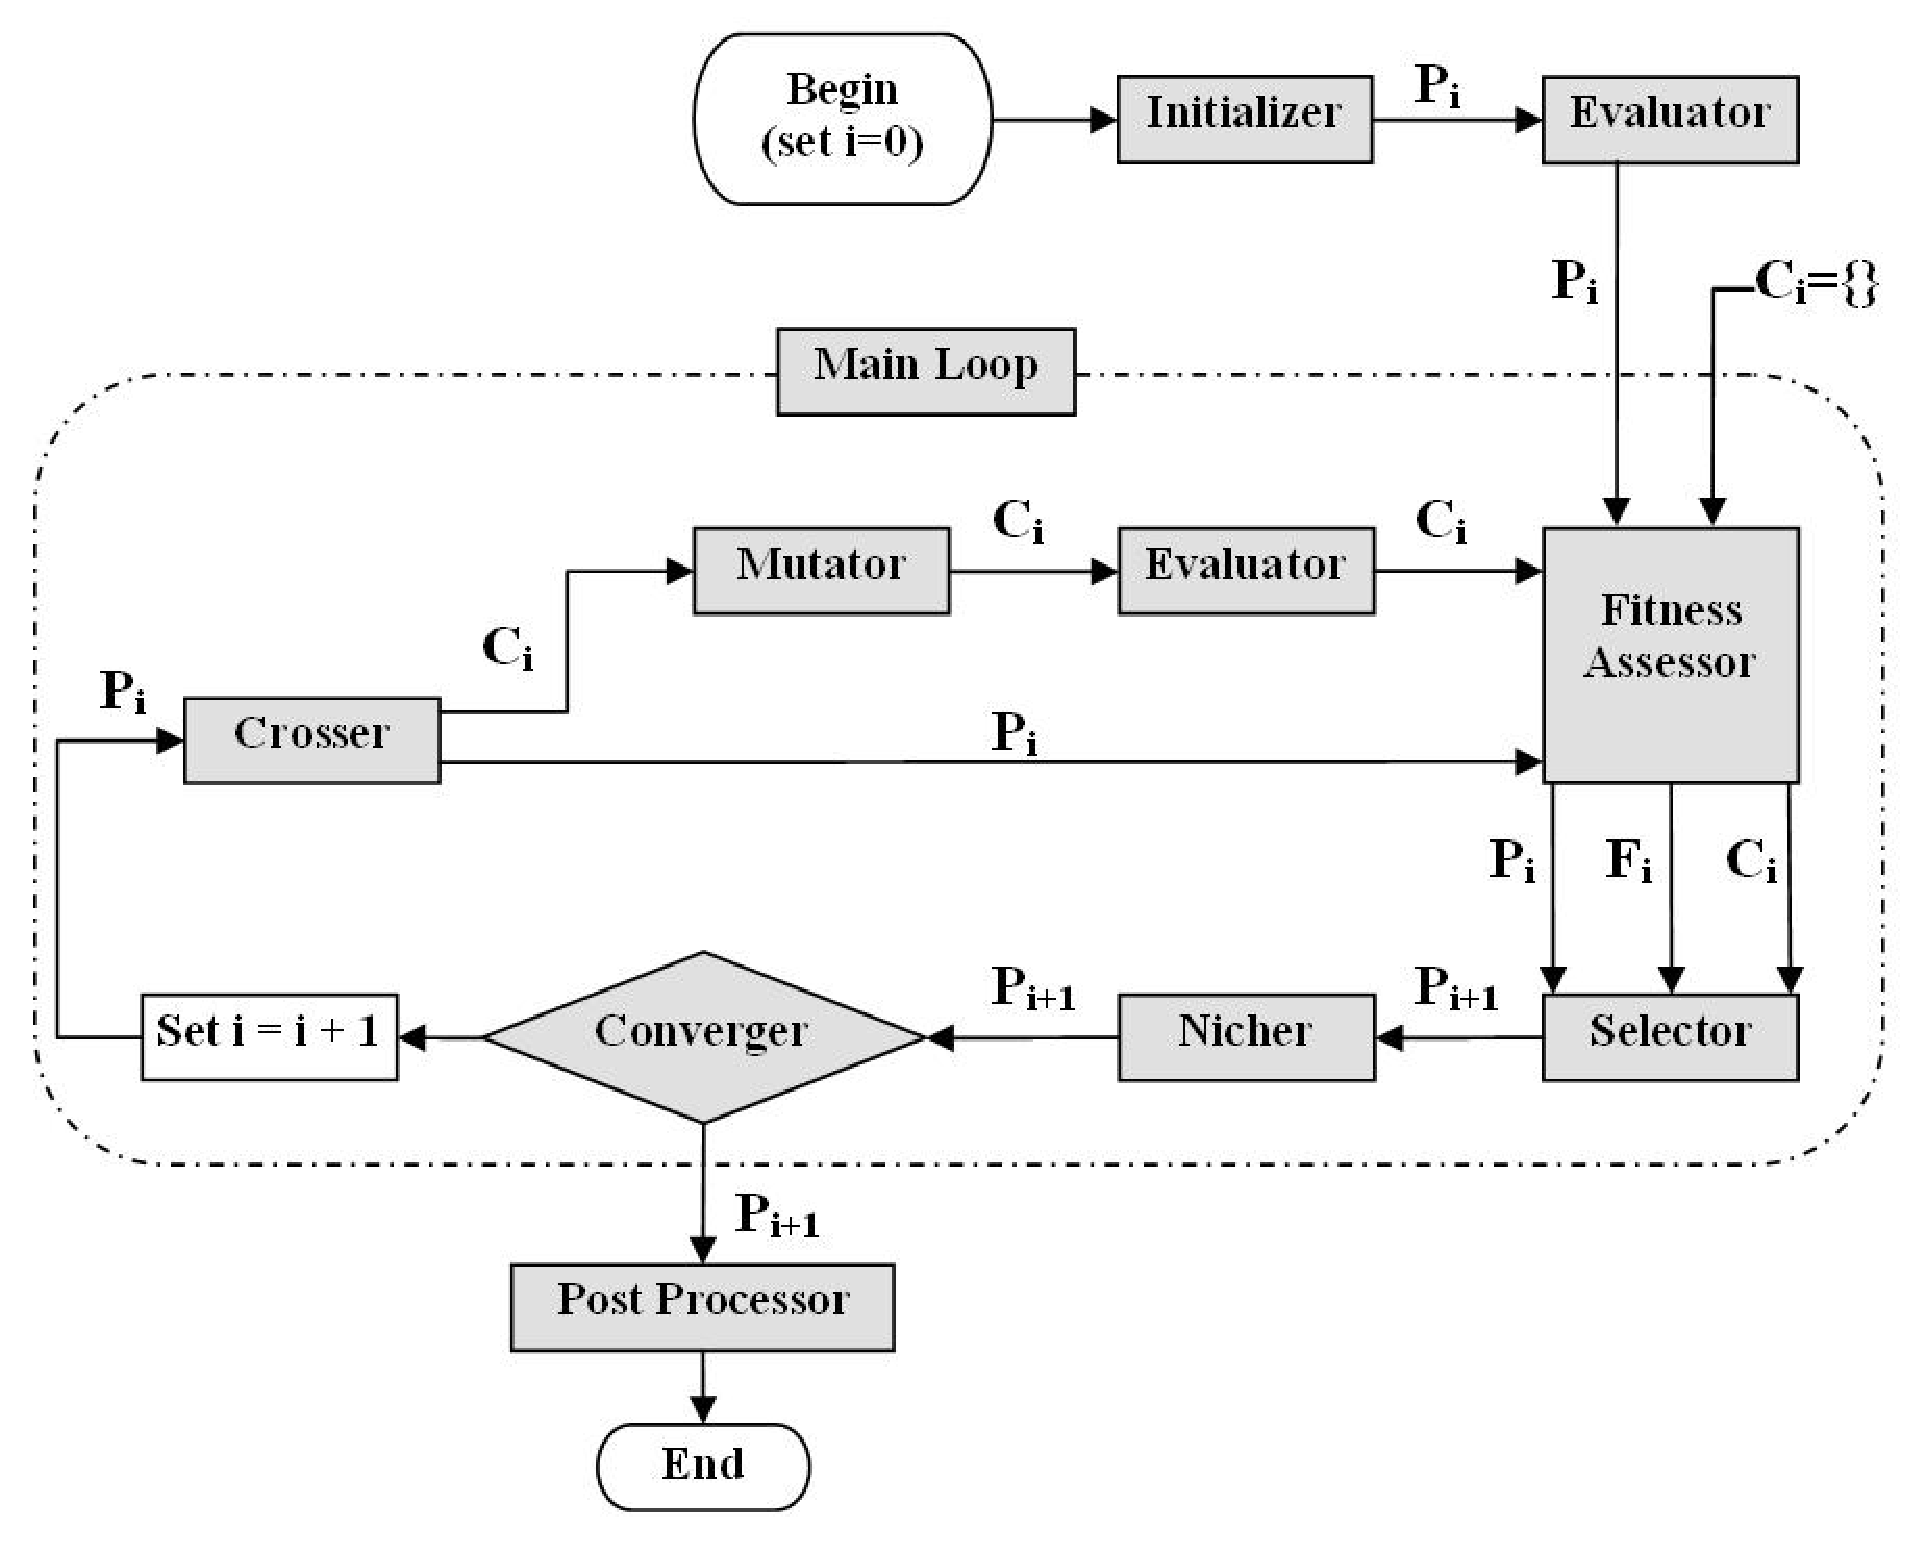
\includegraphics[scale=0.45]{../../images/JEGAFlow.eps}
    \caption{The Typical JEGA Algorithm Progression}
    \label{fig:JEGA_progression}
\end{figure}

In order to inform JEGA what versions of each operator to use, you
must supply it with a string identifier for each. These strings will
be keyed by another string identifier that indicates the class of
operator that is being specified.  The result is a key-value pair
consisting of the operator type identifier followed by the operator
specialization identifier.  So for example, such a pair may have the
form as shown below.  Note that the actual input to JEGA will look
differently because these arguments will be supplied to methods of
the JEGA::FrontEnd::AlgorithmConfig class.

\begin{center}
    $<$"initialization\_type", "unique\_random"$>$
\end{center}

The one exception to this rule is the evaluator which is handled in
a different way as described in Section~\ref{}.
Table~\ref{table:base_operator_inputs} below shows each of the
operator types along with the strings that identify them, the
strings that identify the available specializations common to all
algorithms, and the inputs that are common to all specializations.
In addition to those in this table, there are operator
specializations that are designed specifically for a one or another
algorithm.  Those will be described later.  Note that an input must
be supplied for each operator type meaning that they are all
required.

\subsubsection{Algorithm Independent Inputs}\label{sec:alg_indep_input}
Regardless of which specialization is ultimately chosen for an
operator, in many cases there is information required by the base
class.  This is the information referred to above as being ``common
to all specializations''.  That information is also displayed in
Table~\ref{table:base_operator_inputs}.  Values such as those seen
in the table are specified as triplets whereby a key, type, and
value are all supplied.  An example of such a triplet may have the
form shown below.  Note again that the actual input to JEGA will
look differently.

\begin{center}
    $<$"crossover\_rate", real, 0.8$>$
\end{center}

These values must be supplied (or will be given default values)
regardless of what specialization is chosen.  So for example, no
matter what initializer you choose, you must supply a population
size or be willing to accept the default of 50.

\begin{table}[ht]
    \centering
    {\footnotesize
    \begin{tabular}{|c||l|l|l|l|l|}
      \hline

      \textbf{Operator}                           & \textbf{Identifier}                              & \textbf{Type}           & \textbf{Options}                     & \textbf{Status}           & \textbf{Default} \\ \hline \hline
      \multirow{3}{*}{\textbf{Main Loops}}        & \multirow{3}{*}{method.jega.mainloop\_type}      & \multirow{3}{*}{String} & duplicate\_free                      & \multirow{3}{*}{Required} &                  \\
                                                  &                                                  &                         & null\_main\_loop                     &                           &                  \\
                                                  &                                                  &                         & standard                             &                           &                  \\ \hline
      \multirow{6}{*}{\textbf{Initializers}}      & \multirow{5}{*}{method.initialization\_type}     & \multirow{5}{*}{String} & double\_matrix                       & \multirow{5}{*}{Required} &                  \\
                                                  &                                                  &                         & flat\_file                           &                           &                  \\
                                                  &                                                  &                         & null\_initialization                 &                           &                  \\
                                                  &                                                  &                         & random                               &                           &                  \\
                                                  &                                                  &                         & unique\_random                       &                           &                  \\ \cline{2-6}
                                                  & method.population\_size                          & Integer                 & [0, $\infty$]                        & Optional                  & 50               \\ \hline
      \multirow{7}{*}{\textbf{Mutators}}          & \multirow{6}{*}{method.mutation\_type}           & \multirow{6}{*}{String} & bit\_random                          & \multirow{6}{*}{Required} &                  \\
                                                  &                                                  &                         & null\_mutation                       &                           &                  \\
                                                  &                                                  &                         & offset\_cauchy                       &                           &                  \\
                                                  &                                                  &                         & offset\_normal                       &                           &                  \\
                                                  &                                                  &                         & offset\_uniform                      &                           &                  \\
                                                  &                                                  &                         & replace\_uniform                     &                           &                  \\ \cline{2-6}
                                                  & method.mutation\_rate                            & Real                    & [0.0, 1.0]                           & Optional                  & 0.05             \\ \hline
      \multirow{6}{*}{\textbf{Crossers}}          & \multirow{5}{*}{method.crossover\_type}          & \multirow{5}{*}{String} & multi\_point\_binary                 & \multirow{5}{*}{Required} &                  \\
                                                  &                                                  &                         & multi\_point\_parameterized\_binary  &                           &                  \\
                                                  &                                                  &                         & multi\_point\_real                   &                           &                  \\
                                                  &                                                  &                         & null\_crossover                      &                           &                  \\
                                                  &                                                  &                         & shuffle\_random                      &                           &                  \\ \cline{2-6}
                                                  & method.crossover\_rate                           & Real                    & [0.0, 1.0]                           & Optional                  & 0.75             \\ \hline
      \multirow{8}{*}{\textbf{Convergers}}        & \multirow{6}{*}{method.jega.convergence\_type}   & \multirow{6}{*}{String} & average\_fitness\_tracker            & \multirow{6}{*}{Required} &                  \\
                                                  &                                                  &                         & best\_fitness\_tracker               &                           &                  \\
                                                  &                                                  &                         & max\_evals\_or\_gens                 &                           &                  \\
                                                  &                                                  &                         & max\_evaluations                     &                           &                  \\
                                                  &                                                  &                         & max\_generations                     &                           &                  \\
                                                  &                                                  &                         & null\_convergence                    &                           &                  \\ \cline{2-6}
                                                  & method.max\_iterations                           & Integer                 & [0, $\infty$]                        & Optional                  & $\infty$         \\ \cline{2-6}
                                                  & method.max\_function\_evaluations                & Integer                 & [0, $\infty$]                        & Optional                  & $\infty$         \\ \hline
      \multirow{2}{*}{\textbf{Evaluators}}        &                                                  &                         & \multirow{2}{*}{null\_evaluation}    &                           &                  \\
                                                  &                                                  &                         &                                      &                           &                  \\ \cline{2-6}
                                                  & method.max\_function\_evaluations                & Integer                 & [0, $\infty$]                        & Optional                  & $\infty$         \\ \hline
      \textbf{Fitness}                            & \multirow{2}{*}{method.jega.fitness\_type}       & \multirow{2}{*}{String} & \multirow{2}{*}{null\_fitness}       & \multirow{2}{*}{Required} &                  \\
      \textbf{Assessors}                          &                                                  &                         &                                      &                           &                  \\ \hline
      \multirow{4}{*}{\textbf{Selectors}}         & \multirow{4}{*}{method.replacement\_type}        & \multirow{4}{*}{String} & below\_limit                         & \multirow{4}{*}{Required} &                  \\
                                                  &                                                  &                         & null\_selection                      &                           &                  \\
                                                  &                                                  &                         & roulette\_wheel                      &                           &                  \\
                                                  &                                                  &                         & unique\_roulette\_wheel              &                           &                  \\ \hline
      \multirow{2}{*}{\textbf{Nichers}}           & \multirow{2}{*}{method.jega.niching\_type}       & \multirow{2}{*}{String} & \multirow{2}{*}{null\_niching}       & \multirow{2}{*}{Required} &                  \\
                                                  &                                                  &                         &                                      &                           &                  \\ \cline{2-6}
                                                  & method.jega.cache\_niched\_designs               & Boolean                 & true or false                        & Optional                  & true             \\ \hline
      \textbf{Post}                               & \multirow{2}{*}{method.jega.postprocessor\_type} & \multirow{2}{*}{String} & null\_postprocessor                  & \multirow{2}{*}{Required} &                  \\
      \textbf{Processors}                         &                                                  &                         & distance\_postprocessor              &                           &                  \\ \hline
    \end{tabular}
    }
    \caption{Operator Class Input Requirements.}
    \label{table:base_operator_inputs}
\end{table}

The inputs of the base class will be used by the specializations in
different ways but in general, they have a common meaning.  For
example, the crossover rate will always be used by a crosser to
determine how many crossover operations will take place.  However,
it may be used differently depending on how the operator works. This
will become apparent in Section~\ref{} where the individual operator
specializations are described.

In addition to inputs required for operators, the algorithms
themselves will require inputs.  Again, each algorithm
specialization (MOGA or SOGA) may have specialized requirements but
each will share the requirements of the base class.  The common
algorithm inputs are displayed in
Table~\ref{table:base_algorithm_inputs} below.

\begin{table}[ht]
    \centering
    {\footnotesize
    \begin{tabular}{|l|l|l|l|l|}
      \hline

      \textbf{Identifier}                             & \textbf{Type}             & \textbf{Options}               & \textbf{Status}           & \textbf{Default}                                \\ \hline \hline
      \multirow{2}{*}{method.algorithm}               & \multirow{2}{*}{String}   & moga                           & \multirow{2}{*}{Required} &                                                 \\
                                                      &                           & soga                           &                           &                                                 \\ \hline
      \multirow{2}{*}{method.print\_each\_pop}        & \multirow{2}{*}{Boolean}  & \multirow{2}{*}{true or false} & \multirow{2}{*}{Optional} & \multirow{2}{*}{false}                          \\
                                                      &                           &                                &                           &                                                 \\ \hline
      \multirow{2}{*}{method.jega.algorithm\_name}    & \multirow{2}{*}{String}   &                                & \multirow{2}{*}{Optional} & \multirow{2}{*}{$<$type$>$ \#$<$instance \#$>$} \\
                                                      &                           &                                &                           &                                                 \\ \hline
      \multirow{5}{*}{method.output}                  & \multirow{5}{*}{Integral} & debug   (10)                   & \multirow{5}{*}{Optional} & \multirow{5}{*}{quiet   (30)}                   \\
                                                      &                           & verbose (20)                   &                           &                                                 \\
                                                      &                           & quiet   (30)                   &                           &                                                 \\
                                                      &                           & silent  (40)                   &                           &                                                 \\
                                                      &                           & fatal   (50)                   &                           &                                                 \\ \hline
      \multirow{2}{*}{method.log\_file}               & \multirow{2}{*}{String}   &                                & \multirow{2}{*}{Optional} & \multirow{2}{*}{JEGAGlobal.log}                 \\
                                                      &                           &                                &                           &                                                 \\ \hline
    \end{tabular}
    }
    \caption{Algorithm Class Input Requirements.}
    \label{table:base_algorithm_inputs}
\end{table}

The meanings of these inputs are as follows.  Remember when reading
these descriptions that these inputs pertain to a single algorithm
instance within JEGA.  A single run of JEGA may involve the creation
and marshaling of multiple algorithms.

\begin{itemize}

    \item \textbf{method.algorithm} - Tells JEGA whether to treat
    the problem as a true multi-objective problem and seek the
    Pareto optimal solutions or to treat it as a single objective
    problem and seek the single best solution.  Even if you define
    your problem to have multiple objectives, you can still solve it
    as a single objective problem by supplying JEGA with weights
    with which it can combine the multiple objectives into a single
    objective.  This is a required input and has no default value.
    If not properly supplied, JEGA will cause an exception.

    \item \textbf{method.print\_each\_pop} - Tells JEGA
    whether or not to print the current population after all
    operators in the main loop have been executed at each
    generation.  If this flag is set to true, the populations will
    be written to files with the pattern ``population$<GEN\#>$.dat''
    where $<GEN\#>$ is the number of the current generation.  The
    files will be written in tab delimited format as follows.

    $dv0<tab>dv1...dvN[<tab>of0<tab>of1...ofM<tab>con0<tab>con1...conK]$

    The objectives and constraints are only written if the design
    has been evaluated and is not ill-conditioned.  The constraints
    of course are not written if there are none.  This is an optional
    input with a default value of false meaning that the files will
    not be written.

    \item \textbf{method.jega.algorithm\_name} - Tells JEGA what the
    name of the current algorithm instance is to be.  This if of primary
    use in the creation of logging message.  When information is
    produced for the user by a JEGA algorithm, it is adorned with
    the name of the algorithm that produced it.  This is especially
    important when JEGA is being used to marshal many algorithms
    sequentially or in parallel.  This is an optional input with a
    default value that is constructed based on the algorithm type
    (MOGA or SOGA) and the number of algorithms previously created
    (ex. MOGA \#5).

    \item \textbf{method.output} - Tells JEGA how much output to
    supply to the user.  This input is ignored if logging is not
    enabled.  Each message produced by JEGA is given an importance
    level.  JEGA only outputs those messages whose level is high
    enough compared to the level defined by this input.  The options
    shown in Table~\ref{table:base_operator_inputs} are in order of
    decreasing output.  If you choose the ``debug'' level for
    example, JEGA will write every single message.  If you choose
    ``silent'' on the other hand, JEGA will write almost nothing.
    This is an optional input with a default value of ``quiet''.

    \item \textbf{method.log\_file} - Tells JEGA the name of the
    file to which you would like the current algorithm to log
    messages.  This input is ignored if file logging is not enabled.
    This input is optional and by default, the algorithm will log
    into the global log.

\end{itemize}






















JEGA v2.0 also utilizes the \emph{output} method independent control to
vary the amount of information presented to the user during
execution.

\begin{itemize}
\item Evaluate the new population members.

\item Assess the fitness of each member in the population.  There are
a number of ways to evaluate the fitness of the members of the
populations.  Choice of fitness assessor operators is strongly
dependent on the type of algorithm being used and can have a
profound effect on the choice of selectors.  For example, if using
\emph{MOGA}, the available assessors are the \emph{layer\_rank} and
\emph{domination\_count} fitness assessors.  If using either of
these, it is strongly recommended that you use the
\emph{below\_limit} selector as well (although the roulette wheel
selectors can also be used).  The functionality of the
\emph{dominationr\_count} selector of JEGA v1.0 can now be achieved
using the \emph{domination\_count} fitness assessor and
\emph{below\_limit} selector together.  If using \emph{SOGA}, the
only fitness assessor is the \emph{merit\_function} fitness assessor
which currently uses an exterior penalty function formulation to
assign fitnesses. Any of the selectors can be used in conjunction
with this fitness assessment scheme.  This is the first of the
selection operators.

\item Replace the population with members selected to continue in the
next generation.  The pool of potential members is the current
population and the current set of offspring.  The
\emph{replacement\_type} of \emph{roulette\_wheel} or
\emph{unique\_roulette\_wheel} may be used either with MOGA or SOGA
problems however they are not recommended for use with MOGA.  Given
that the only two fitness assessors for MOGA are the
\emph{layer\_rank} and \emph{domination\_count}, the recommended
selector is the \emph{below\_limit} selector. The
\emph{replacement\_type} of \emph{favor\_feasible} is specific to a
SOGA. This replacement operator will always take a feasible design
over an infeasible one.  Beyond that, it favors solutions based on
an assigned fitness value which must have been installed by some
fitness assessor.

\item Apply niche pressure to the population.  This step is specific
to the MOGA and is new to JEGA v2.0.  Technically, the step is
carried out during runs of the SOGA but only the
\emph{null\_niching} operator is available for use with SOGA.  In
MOGA, the \emph{radial} niching operator or the \emph{distance}
niching operator can be used. The purpose of niching is to encourage
differentiation along the Pareto frontier and thus a more even and
uniform sampling.  In JEGA, niching operators typically work by
determining when two designs are too close in the performance
(phenotype) space and caching them until the next round of
selection.

\item Test for convergence.  The final step in the iterator loop is
to assess the convergence of the algorithm.  There are two aspects
to convergence that must be considered.  The first is stopping
criteria.  A stopping criteria dictates some sort of limit on the
algorithm that is independent of its performance.  Examples of
stopping criteria available for use with JEGA are the
\emph{max\_iterations} and \emph{max\_function\_evaluations} inputs.
All JEGA convergers respect these stopping criteria in addition to
anything else that they do.

The second aspect to convergence involves repeated assessment of the
algorithms progress in solving the problem.  In JEGA v1.0, the
fitness tracker convergers (\emph{best\_fitness\_tracker} and
\emph{average\_fitness\_tracker}) performed this function by
asserting that the fitness values (either best or average) of the
population continue to improve.  There was no such operator for the
MOGA.  As of JEGA v2.0, the same fitness tracker convergers exist
for use with SOGA and there is now a converger available for use
with the MOGA. The MOGA converger (\emph{metric\_tracker}) operates
by tracking various changes in the non-dominated frontier from
generation to generation. When the changes occurring over a user
specified number of generations fall below a user specified
threshold, the algorithm stops.

\item Post Process.  This occurs after convergence has been
attained.  This operator provides a means of filtering the data
returned by the algorithm in whatever way is relevant.  For example,
if using a MOGA, it may be desired to return only a certain number
of points within a particular region or evenly dispersed throughout
the performance space, etc.
\end{itemize}

There are many controls which can be used for both MOGA and SOGA
methods.  These include among others the random seed, initialization
types, crossover and mutation types, and some replacement types.

The \emph{seed} control defines the starting seed for the random
number generator.  The algorithm uses random numbers heavily but a
specification of a random seed will cause the algorithm to run
identically from one trial to the next so long as all other input
specifications remain the same.  New to JEGA v2.0 is the
introduction of the \emph{log\_file} specification.  JEGA v2.0 uses
a logging library to output messages and status to the user.  JEGA
can be configured at build time to log to both standard error and a
text file, one or the other, or neither.  The \emph{log\_file} input
is a string name of a file into which to log.  If the build was
configured without file logging in JEGA, this input is ignored.  If
file logging is enabled and no \emph{log\_file} is specified, the
default file name if JEGAGlobal.log is used.  Also new to JEGA v2.0
is the introduction of the \emph{print\_each\_pop} specification. It
serves as a flag and if supplied, the population at each generation
will be printed to a file named ``population$<GEN\#>$.dat'' where
$<GEN\#>$ is the number of the current generation.

The \emph{initialization\_type} defines the type of initialization
for the GA.  There are three types: \emph{simple\_random},
\emph{unique\_random}, and \emph{flat\_file}.  \emph{simple\_random}
creates initial solutions with random variable values according to a
uniform random number distribution. It gives no consideration to any
previously generated designs.  The number of designs is specified by
the \emph{population\_size}. \emph{unique\_random} is the same as
\emph{simple\_random}, except that when a new solution is generated,
it is checked against the rest of the solutions.  If it duplicates
any of them, it is rejected.  \emph{flat\_file} allows the initial
population to be read from a flat file.  If \emph{flat\_file} is
specified, a file name must be given.

Variables can be delimited in the flat file in any way you see fit
with a few exceptions.  The delimiter must be the same on any given
line of input with the exception of leading and trailing whitespace.
So a line could look like: 1.1, 2.2  ,3.3 for example but could not
look like: 1.1, 2.2  3.3.  The delimiter can vary from line to line
within the file which can be useful if data from multiple sources is
pasted into the same input file. The delimiter can be any string
that does not contain any of the characters .+-dDeE or any of the
digits 0-9.  The input will be read until the end of the file.  The
algorithm will discard any configurations for which it was unable to
retrieve at least the number of design variables.  The objective and
constraint entries are not required but if ALL are present, they
will be recorded and the design will be tagged as evaluated so that
evaluators may choose not to re-evaluate them.  Setting the size for
this initializer has the effect of requiring a minimum number of
designs to create.  If this minimum number has not been created once
the files are all read, the rest are created using the
\emph{unique\_random} initializer and then the \emph{simple\_random}
initializer if necessary.

Note that the \emph{population\_size} only sets the size of the
initial population.  The population size may vary in the JEGA
methods according to the type of operators chosen for a particular
optimization run.

There are many crossover types available.
\emph{multi\_point\_binary} crossover requires an integer number, N,
of crossover points.  This crossover type performs a bit switching
crossover at N crossover points in the binary encoded genome of two
designs.  Thus, crossover may occur at any point along a solution
chromosome (in the middle of a gene representing a design variable,
for example). \emph{multi\_point\_parameterized\_binary} crossover
is similar in that it performs a bit switching crossover routine at
N crossover points. However, this crossover type performs crossover
on each design variable individually. So the individual chromosomes
are crossed at N locations. \emph{multi\_point\_real} crossover
performs a variable switching crossover routing at N crossover
points in the real real valued genome of two designs. In this
scheme, crossover only occurs between design variables
(chromosomes).  Note that the standard solution chromosome
representation in the JEGA algorithm is real encoded and can handle
integer or real design variables.  For any crossover types that use
a binary representation, real variables are converted to long
integers by multiplying the real number by $10^6$ and then
truncating. Note that this assumes a precision of only six decimal
places. Discrete variables are represented as integers (indices
within a list of possible values) within the algorithm and thus
require no special treatment by the binary operators.

The final crossover type is \emph{shuffle\_random}.  This crossover
type performs crossover by choosing design variables at random from
a specified number of parents enough times that the requested number
of children are produced.  For example, consider the case of 3
parents producing 2 children.  This operator would go through and
for each design variable, select one of the parents as the donor for
the child. So it creates a random shuffle of the parent design
variable values. The relative numbers of children and parents are
controllable to allow for as much mixing as desired.  The more
parents involved, the less likely that the children will wind up
exact duplicates of the parents.

All crossover types take a \emph{crossover\_rate}.  The crossover
rate is used to calculate the number of crossover operations that
take place. The number of crossovers is equal to the rate *
\emph{population\_size}.

There are five mutation types allowed.  \emph{replace\_uniform}
introduces random variation by first randomly choosing a design
variable of a randomly selected design and reassigning it to a
random valid value for that variable.  No consideration of the
current value is given when determining the new value.  All mutation
types have a \emph{mutation\_rate}.  The number of mutations for the
\emph{replace\_uniform} mutator is the product of the
\emph{mutation\_rate} and the \emph{population\_size}.

The \emph{bit\_random} mutator introduces random variation by first
converting a randomly chosen variable of a randomly chosen design
into a binary string.  It then flips a randomly chosen bit in the
string from a 1 to a 0 or visa versa. In this mutation scheme, the
resulting value has more probability of being similar to the
original value.  The number of mutations performed is the product of
the \emph{mutation\_rate}, the number of design variables, and the
\emph{population\_size}.

The offset mutators all act by adding an ``offset'' random amount to
a variable value.  The random amount has a mean of zero in all
cases. The \emph{offset\_normal} mutator introduces random variation
by adding a Gaussian random amount to a variable value.  The random
amount has a standard deviation dependent on the
\emph{mutation\_scale}.  The \emph{mutation\_scale} is a fraction in
the range [0, 1] and is meant to help control the amount of
variation that takes place when a variable is mutated.
\emph{mutation\_scale} is multiplied by the range of the variable
being mutated to serve as standard deviation. \emph{offset\_cauchy}
is similar to \emph{offset\_normal}, except that a Cauchy random
variable is added to the variable being mutated.  The
\emph{mutation\_scale} also defines the standard deviation for this
mutator. Finally, \emph{offset\_uniform} adds a uniform random
amount to the variable value.  For the \emph{offset\_uniform}
mutator, the \emph{mutation\_scale} is interpreted as a fraction of
the total range of the variable.  The range of possible deviation
amounts is +/- 1/2 * (\emph{mutation\_scale} * variable range).  The
number of mutations for all offset mutators is defined as the
product of \emph{mutation\_rate} and \emph{population\_size}.

As of JEGA v2.0, all replacement types are common to both MOGA and
SOGA. They include the \emph{roulette\_wheel},
\emph{unique\_roulette\_wheel}, and \emph{below\_limit} selectors.
In \emph{roulette\_wheel replacement}, each design is conceptually
allotted a portion of a wheel proportional to its fitness relative
to the fitnesses of the other Designs.  Then, portions of the wheel
are chosen at random and the design occupying those portions are
duplicated into the next population.  Those Designs allotted larger
portions of the wheel are more likely to be selected (potentially
many times). \emph{unique\_roulette\_wheel} replacement is the same
as \emph{roulette\_wheel} replacement, with the exception that a
design may only be selected once.  The \emph{below\_limit} selector
attempts to keep all designs for which the negated fitness is below
a certain limit.  The values are negated to keep with the convention
that higher fitness is better. The inputs to the \emph{below\_limit}
selector are the limit as a real value, and a
\emph{shrinkage\_percentage} as a real value.  The
\emph{shrinkage\_percentage} defines the minimum amount of
selections that will take place if enough designs are available.  It
is interpreted as a percentage of the population size that must go
on to the subsequent generation.  To enforce this,
\emph{below\_limit} makes all the selections it would make anyway
and if that is not enough, it takes the remaining that it needs from
the best of what is left (effectively raising its limit as far as it
must to get the minimum number of selections).  It continues until
it has made enough selections.  The \emph{shrinkage\_percentage} is
designed to prevent extreme decreases in the population size at any
given generation, and thus prevent a big loss of genetic diversity
in a very short time.  Without a shrinkage limit, a small group of
``super'' designs may appear and quickly cull the population down to
a size on the order of the limiting value.  In this case, all the
diversity of the population is lost and it is expensive to
re-diversify and spread the population.
%
%\anchor T5d17 <table> <caption align = "top"> \htmlonly Table 5.17
%\endhtmlonly
%Specification detail for JEGA method dependent controls: seed,
%output, initialization, mutation, and replacement </caption> <tr>
%<td><b>Description</b> <td><b>Keyword</b> <td><b>Associated Data</b>
%<td><b>Status</b> <td><b>Default</b> <tr> <td>GA Method
%<td>\emph{moga}| \emph{soga} <td>none <td>Required group <td>N/A
%<tr> <td>Random Seed <td>\emph{seed} <td>integer <td>Optional
%<td>Time based seed <tr> <td>Log File <td>\emph{log\_file} <td>string
%<td>Optional <td>JEGAGlobal.log <tr> <td>Population Output
%<td>\emph{print\_each\_pop} <td>none <td>Optional <td>N/A <tr>
%<td>Output verbosity <td>\emph{output} <td>\emph{silent} |
%\emph{quiet} | \emph{verbose} | \emph{debug} <td>Optional
%<td>\emph{normal} <tr> <td>Initialization type
%<td>\emph{initialization\_type} <td>\emph{simple\_random} |
%\emph{unique\_random} | \emph{flat\_file} <td>Required
%<td>unique\_random <tr> <td>Mutation type <td>\emph{mutation\_type}
%<td>\emph{replace\_uniform} | \emph{bit\_random} |
%\emph{offset\_cauchy} | \emph{offset\_uniform} | \emph{offset\_normal}
%<td>Optional group <td>None <tr> <td>Mutation scale
%<td>\emph{mutation\_scale} <td>real <td>Optional <td>0.15 <tr>
%<td>Mutation rate <td>\emph{mutation\_rate} <td>real <td>Optional
%<td>0.08 <tr> <td>Replacement type <td>\emph{replacement\_type}
%<td>\emph{below\_limit} | \emph{roulette\_wheel} |
%\emph{unique\_roulette\_wheel} <td>Required group <td>None <tr>
%<td>Below limit selection <td>\emph{below\_limit} <td>real
%<td>Optional <td>6 <tr> <td>Shrinkage percentage in below limit
%selection <td>\emph{shrinkage\_percentage} <td>real <td>Optional<BR>
%<td>0.9 </table>


%
%</table>
%
%\anchor T5d18 <table> <caption align = "top"> \htmlonly Table 5.18
%\endhtmlonly
%Specification detail for JEGA method dependent controls: crossover
%</caption> <tr> <td><b>Description</b> <td><b>Keyword</b>
%<td><b>Associated Data</b> <td><b>Status</b> <td><b>Default</b> <tr>
%<td>Crossover type <td>\emph{crossover\_type} <td>\emph{multi\_point\_binary} |
%\emph{multi\_point\_parameterized\_binary} |
%    \emph{multi\_point\_real} | \emph{shuffle\_random}
%<td>Optional group <td>none <tr> <td>Multi point binary crossover
%<td>\emph{multi\_point\_binary} <td>integer <td>Required <td>N/A <tr>
%<td>Multi point parameterized binary crossover <td>\c
%multi\_point\_parameterized\_binary <td>integer <td>Required <td>N/A
%<tr> <td>Multi point real crossover <td>\emph{multi\_point\_real}
%<td>integer <td>Required <td>N/A <tr> <td>Random shuffle crossover
%<td>\emph{shuffle\_random} <td>\emph{num\_parents}, \emph{num\_offspring}
%<td>Required <td>N/A <tr> <td>Number of parents in random shuffle
%crossover <td>\emph{num\_parents} <td>integer <td>optional <td>2 <tr>
%<td>Number of offspring in random shuffle crossover <td>\c
%num\_offspring <td>integer <td>optional <td>2 <tr> <td>Crossover rate
%<td>\emph{crossover\_rate} <td>real <td>optional (applies to all
%crossover types) <td>0.8 </table>

%\subsection MethodJEGAMOGA Multi-objective Evolutionary Algorithms

The specification for controls specific to Multi-objective
Evolutionary algorithms are described here.  These controls will be
appropriate to use if the user has specified \emph{moga} as the method.

The initialization, crossover, and mutation controls were all
described in the preceding section.  There are no MOGA specific
aspects to these controls.  The \emph{fitness\_type} for a MOGA may
be \emph{domination\_count} or \emph{layer\_rank}.  Both have been
specifically designed to avoid problems with aggregating and scaling
objective function values and transforming them into a single
objective. Instead, the \emph{domination\_count} fitness assessor
works by ordering population members by the negative of the number
of designs that dominate them.  The values are negated in keeping
with the convention that higher fitness is better.  The
\emph{layer\_rank} fitness assessor works by assigning all
non-dominated designs a layer of 0, then from what remains,
assigning all the non-dominated a layer of -1, and so on until all
designs have been assigned a layer.  Again, the values are negated
for the higher-is-better fitness convention. Use of the
\emph{below\_limit} selector with the \emph{domination\_count}
fitness assessor has the effect of keeping all designs that are
dominated by fewer then a limiting number of other designs subject
to the shrinkage limit.  Using it with the \emph{layer\_rank}
fitness assessor has the effect of keeping all those designs whose
layer is below a certain threshold again subject to a minimum.

New to JEGA v2.0 is the introduction of niche pressure operators.
These operators are meant primarily for use with the moga.  The job
of a niche pressure operator is to encourage diversity along the
Pareto frontier as the algorithm runs.  This is typically
accomplished by discouraging clustering of design points in the
performance space.  In JEGA, the application of niche pressure
occurs as a secondary selection operation.  The nicher is given a
chance to perform a pre-selection operation prior to the operation
of the selection (replacement) operator, and is then called to
perform niching on the set of designs that were selected by the
selection operator.

Currently, the only niche pressure operator available is the
\emph{radial} nicher. This niche pressure applicator works by
enforcing a minimum distance between designs in the performance
space at each generation.  The algorithm proceeds by starting at the
(or one of the) extreme designs along objective dimension 0 and
marching through the population removing all designs that are too
close to the current design.  One exception to the rule is that the
algorithm will never remove an extreme design which is defined as a
design that is maximal or minimal in all but 1 objective dimension
(for a classical 2 objective problem, the extreme designs are those
at the tips of the non-dominated frontier).

The designs that are removed by the nicher are not discarded.  They
are buffered and re-inserted into the population during the next
pre-selection operation.  This way, the selector is still the only
operator that discards designs and the algorithm will not waste time
``re-filling'' gaps created by the nicher.

The niche pressure control consists of two options.  The first is
the \emph{null\_niching} option which specifies that no niche
pressure is to be applied. The second is the \emph{radial\_niching}
option which specifies that the radial niching algorithm is to be
use.  The radial nicher requires as input a vector of fractions with
length equal to the number of objectives.  The elements of the
vector are interpreted as percentages of the non-dominated range for
each objective defining a minimum distance to all other designs. All
values should be in the range (0, 1).  The minimum allowable
distance between any two designs in the performance space is the
euclidian distance defined by these percentages.

Also new to JEGA v2.0 is the introduction of the MOGA specific
\emph{metric\_tracker} converger.  This converger is conceptually
similar to the best and average fitness tracker convergers in that
it tracks the progress of the population over a certain number of
generations and stops when the progress falls below a certain
threshold.  The implementation is quite different however.  The
\emph{metric\_tracker} converger tracks 3 metrics specific to the
non-dominated frontier from generation to generation.  All 3 of
these metrics are computed as percent changes between the
generations.  In order to compute these metrics, the converger
stores a duplicate of the non-dominated frontier at each generation
for comparison to the non-dominated frontier of the next generation.

The first metric is one that indicates how the expanse of the
frontier is changing.  The expanse along a given objective is
defined by the range of values existing within the non-dominated
set.  The expansion metric is computed by tracking the extremes of
the non-dominated frontier from one generation to the next.  Any
movement of the extreme values is noticed and the maximum percentage
movement is computed as:

\begin{equation}\label{eq:pareto_expansion}
    E_m = \max_{j=1}^{nof} |\frac{range(j, i) - range(j, i-1)}{range(j, i-1)}|
\end{equation}

where $E_m$ is the max expansion metric, $j$ is the objective function
index, $i$ is the current generation number, and $nof$ is the
total number of objectives.  The range is the difference between the
largest value along an objective and the smallest when considering
only non-dominated designs.

The second metric monitors changes in the density of the
non-dominated set.  The density metric is computed as the number of
non-dominated points divided by the hypervolume of the non-dominated
region of space.  Therefore, changes in the density can be caused by
changes in the number of non-dominated points or by changes in size
of the non-dominated space or both.  The size of the non-dominated
space is computed as:

\begin{equation}\label{eq:pareto_hypervolume}
    V_{ps}(i) = \prod_{j=1}^{nof} range(j, i)
\end{equation}

where $V_{ps}(i)$ is the hypervolume of the non-dominated space at
generation $i$ and all other terms have the same meanings as above.

The density of the a given non-dominated space is then:

\begin{equation}\label{eq:pareto_density}
    D_{ps}(i) = \frac{P_{ct}(i)}{V_{ps}(i)}
\end{equation}

where $P_{ct}(i)$ is the number of points on the non-dominated frontier
at generation $i$.

The percentage increase in density of the frontier is then
calculated as:

\begin{equation}
    C_d = | \frac{D_{ps}(i) - D_{ps}(i-1)}{D_{ps}(i-1)}|
\end{equation}

where $C_d$ is the change in density metric.

The final metric is one that monitors the ``goodness'' of the
non-dominated frontier.  This metric is computed by considering each
design in the previous population and determining if it is dominated
by any designs in the current population.  All that are determined
to be dominated are counted. The metric is the ratio of the number
that are dominated to the total number that exist in the previous
population.

As mentioned above, each of these metrics is a percentage.  The
tracker records the largest of these three at each generation.  Once
the recorded percentage is below the supplied percent change for the
supplied number of generations consecutively, the algorithm is
converged.

The specification for convergence in a MOGA can either be
\emph{metric\_tracker} or can be omitted all together.  If omitted,
no convergence algorithm will be used and the algorithm will rely on
stopping criteria only.  If \emph{metric\_tracker} is specified,
then a \emph{percent\_change} and \emph{num\_generations} must be
supplied as with the other metric tracker convergers (average and
best fitness trackers).  The \emph{percent\_change} is the threshold
beneath which convergence is attained whereby it is compared to the
metric value computed as described above.  The
\emph{num\_generations} is the number of generations over which the
metric value should be tracked. Convergence will be attained if the
recorded metric is below \emph{percent\_change} for
\emph{num\_generations} consecutive generations.

The MOGA specific controls are described in %\ref T5d19 "Table 5.19"
below. Note that MOGA and SOGA create additional output files during
execution.  ``finaldata.dat'' is a file that holds the Pareto
members of the population in the final generation.  ``discards.dat''
holds solutions that were discarded from the population during the
course of evolution. It can often be useful to plot objective
function values from these files to visually see the Pareto front
and ensure that finaldata.dat solutions dominate discards.dat
solutions.  The solutions are written to these output files in the
format ``Input1...InputN..Output1...OutputM''. If MOGA is used in a
multi-level optimization strategy (which requires one optimal
solution from each individual optimization method to be passed to
the subsequent optimization method as its starting point), the
solution in the Pareto set closest to the ``utopia'' point is given
as the best solution. This solution is also reported in the DAKOTA
output. This ``best'' solution in the Pareto set has minimum
distance from the utopia point.  The utopia point is defined as the
point of extreme (best) values for each objective function.  For
example, if the Pareto front is bounded by (1,100) and (90,2), then
(1,2) is the utopia point.  There will be a point in the Pareto set
that has minimum L2-norm distance to this point, for example (10,10)
may be such a point.  In SOGA, the solution that minimizes the
single objective function is returned as the best solution.

%
%\anchor T5d19 <table> <caption align = "top"> \htmlonly Table 5.19
%\endhtmlonly
%Specification detail for MOGA method controls </caption> <tr>
%<td><b>Description</b> <td><b>Keyword</b> <td><b>Associated Data</b>
%<td><b>Status</b> <td><b>Default</b> <tr> <td>Fitness type
%<td>\emph{fitness\_type} <td>\emph{layer\_rank} |
%\emph{domination\_count} <td>Required group <td> None <tr> <td>Niche
%pressure type <td>\emph{niching\_type} <td>\emph{radial\_niching}
%<td>Optional group <td> No niche pressure <tr> <td>Radial niching
%<td>\emph{radial\_niching} <td>list of real <td>Optional <td> 0.01
%for all objectives <tr> <td>Convergence type
%<td>\emph{metric\_tracker} <td>none <td>Optional group <td>Stopping
%criteria only <tr> <td>Percent change limit for metric\_tracker
%converger <td>\emph{percent\_change} <td>real <td>Optional <td>0.1
%<tr> <td>Number generations for metric\_tracker converger
%<td>\emph{num\_generations} <td>integer <td>Optional <td>10 </table>


%\subsection MethodJEGASOGA Single-objective Evolutionary Algorithms

The specification for controls specific to Single-objective
Evolutionary algorithms are described here.  These controls will be
appropriate to use if the user has specified \emph{soga} as the method.

The initialization, crossover, and mutation controls were all
described above.  There are no SOGA specific aspects to these
controls.  The \emph{replacement\_type} for a SOGA may be
\emph{roulette\_wheel}, \emph{unique\_roulette\_wheel}, or
\emph{favor\_feasible}.  The \emph{favor\_feasible} replacement type
always takes a feasible design over an infeasible one. Beyond that,
it selects designs based on a fitness value.  As of JEGA v2.0, the
fitness assessment operator must be specified with SOGA although the
\emph{merit\_function} is currently the only one.  The roulette
wheel selectors no longer assume a fitness function.  The
\emph{merit\_function} fitness assessor uses an exterior penalty
function formulation to penalize infeasible designs.  The
specification allows the input of a \emph{constraint\_penalty} which
is the multiplier to use on the constraint violations.

The SOGA controls allow two additional convergence types.  The
\emph{convergence\_type} called \emph{average\_fitness\_tracker}
keeps track of the average fitness in a population.  If this average
fitness does not change more than \emph{percent\_change} over some
number of generations, \emph{num\_generations}, then the solution is
reported as converged and the algorithm terminates. The
\emph{best\_fitness\_tracker} works in a similar manner, only it
tracks the best fitness in the population. Convergence occurs after
\emph{num\_generations} has passed and there has been less than
\emph{percent\_change} in the best fitness value.  Both also respect
the stopping criteria.

The SOGA specific controls are described in %\ref T5d20 "Table 5.20"
below.
%
%\anchor T5d20 <table> <caption align = "top"> \htmlonly Table 5.20
%\endhtmlonly
%Specification detail for SOGA method controls </caption> <tr>
%<td><b>Description</b> <td><b>Keyword</b> <td><b>Associated Data</b>
%<td><b>Status</b> <td><b>Default</b> <tr> <td>Fitness type
%<td>\emph{fitness\_type} <td>\emph{merit\_function} <td>Optional group
%<td> merit\_function <tr> <td>Merit function fitness
%<td>\emph{merit\_function} <td>\emph{real} <td>Optional <td>1.0 <tr>
%<td>Replacement type <td>\emph{replacement\_type}
%<td>\emph{favor\_feasible} | \emph{unique\_roulette\_wheel} |
%\emph{roulette\_wheel} <td>Optional group <td> <tr> <td>Convergence
%type <td>\emph{convergence\_type} <td>\emph{best\_fitness\_tracker} |
%\emph{average\_fitness\_tracker} <td>Optional <td> <tr> <td>Number of
%generations (for convergence test) <td>\emph{num\_generations}
%<td>integer <td>Optional <td>10 <tr> <td>Percent change in fitness
%<td>\emph{percent\_change} <td>real <td>Optional <td>0.1 </table>
